\begin{figure}[H]
  \centering

  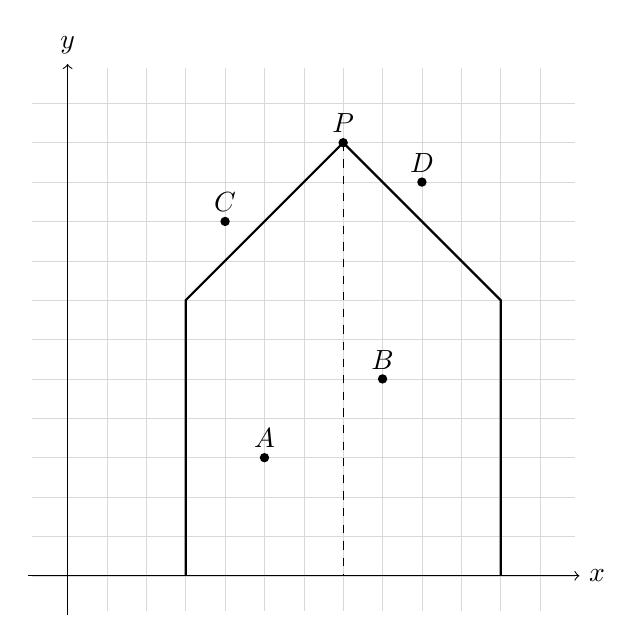
\begin{tikzpicture}[
    point/.style = { circle, fill, inner sep=1.2pt },
    ]

    % axes
    \draw[help lines, color=gray!30, step=0.5] (-0.45, -0.45) grid (6.45, 6.45);
    \draw[->] (-0.5,0)--(6.5,0) node[right]{$x$};
    \draw[->] (0,-0.5)--(0,6.5) node[above]{$y$};

    \coordinate[label=above:$P$] (P) at (3.5, 5.5);
    \coordinate[label=above:$A$] (A) at (2.5, 1.5);
    \coordinate[label=above:$B$] (B) at (4.0, 2.5);
    \coordinate[label=above:$C$] (C) at (2.0, 4.5);
    \coordinate[label=above:$D$] (D) at (4.5, 5.0);
    \node[point] at (P) {};
    \node[point] at (A) {};
    \node[point] at (B) {};
    \node[point] at (C) {};
    \node[point] at (D) {};

    \draw[thick] (1.5, 0) -- (1.5, 3.5) -- (P) -- (5.5, 3.5) -- (5.5, 0);
    \draw[dashed] (P) -- (3.5, 0);

  \end{tikzpicture}

  \caption{Zona de acoperire a festivalului $P$ pentru $d = 4$. Punctul $P$ poate fi vizitat după punctele $A$ sau $B$, dar nu și după $C$ sau $D$.}
  \label{fig:offline-2d-festival}
\end{figure}
